\documentclass{beamer}
\usepackage{ctex, hyperref}
\usepackage[T1]{fontenc}

% other packages
\usepackage{latexsym,amsmath,xcolor,multicol,booktabs,calligra}
\usepackage{graphicx,pstricks,listings,stackengine}
\usepackage[normalem]{ulem}
\usepackage{tikz}
\author{userElaina, Misaka, TechCiel}
\title{Linux Install Party!}
\institute{吉林大学 Linux 用户协会}
\date{2025.04.26 (春季学期)}
\usepackage{JilinUniv}

\def\cmd#1{\texttt{\color{red}\footnotesize $\backslash$#1}}
\def\env#1{\texttt{\color{blue}\footnotesize #1}}
\definecolor{deepblue}{rgb}{0,0,0.5}
\definecolor{deepred}{rgb}{0.6,0,0}
\definecolor{deepgreen}{rgb}{0,0.5,0}
\definecolor{halfgray}{gray}{0.55}

\lstset{
    basicstyle=\ttfamily\small,
    keywordstyle=\bfseries\color{deepblue},
    emphstyle=\ttfamily\color{deepred},    % Custom highlighting style
    stringstyle=\color{deepgreen},
    numbers=left,
    numberstyle=\small\color{halfgray},
    rulesepcolor=\color{red!20!green!20!blue!20},
    frame=shadowbox,
}

\begin{document}

\kaishu
\begin{frame}
    \titlepage
    \begin{figure}[htpb]
        \begin{center}
            
\includegraphics[width=0.15\linewidth]{pic/Jilin_University_Logo.eps}
        \end{center}
    \end{figure}
\end{frame}

\begin{frame}
\tableofcontents[sectionstyle=show,subsectionstyle=show/shaded/hide,subsubsectionstyle=show/shaded/hide]
\end{frame}

% \textbf{2024 春季学期 4月 26日 18:30 @ 中心逸夫 207 吉林大学 Linux 用户协会}

\section{自由软件与 GNU/Linux 简史}

\begin{frame}{UNIX}
    \begin{itemize}
        \item 1969 年, 贝尔实验室开发了 UNIX 操作系统并开源, 得到了广泛的应用.
        \item 但随后改变了策略, 推行许可证, 并开始打版权官司.
    \end{itemize}
\end{frame}

\begin{frame}{\textbf{G}NU is \textbf{N}ot \textbf{U}nix!}
\begin{columns}
\begin{column}{0.8\textwidth}
    \begin{itemize}
        \item 1983 年, Richard M. Stallman 不满软件产业封闭和保护的转变, 毅然离开 MIT 发起了 GNU 计划, 希望创建一个类似 UNIX 但完全自由的操作系统.
        \item \texttt{为了能够不失尊严地继续使用计算机, 我决定把一些必要的自由软件集合在一起, 这样我就不再需要任何不自由的软件.}
        \item 一个自由软件允许用户自由地运行, 拷贝, 分发, 学习, 修改并改进该软件.
        \item GNU General Public License (GNU 通用公共许可证), GNU bash, GNU Emacs, GNU Compiler Collection (GCC).
    \end{itemize}
\end{column}
\begin{column}{0.2\textwidth}
    \begin{figure}[c]
        \centering
        
\includegraphics[width=\textwidth]{pic/gnu.png}
    \end{figure}
\end{column}
\end{columns}
\end{frame}

\begin{frame}{Linux Kernel}
\begin{columns}
\begin{column}{0.8\textwidth}
    \begin{itemize}
        \item 截至 1991 年, GNU Hurd 几乎一直处于搁置状态.
        \item 彼时, 21 岁的 Linus Torvalds 在芬兰赫尔辛基大学读大三. 他不满意 MINIX 只能用于教育, 于是自己开发了最初的 Linux 内核.
        \item \texttt{just a hobby, won't be big and professional like GNU}
    \end{itemize}
\end{column}
\begin{column}{0.2\textwidth}
    \begin{figure}[c]
        \centering
        
\includegraphics[width=\textwidth]{pic/tux.png}
    \end{figure}
\end{column}
\end{columns}
\end{frame}

\begin{frame}{GNU/Linux}
    \begin{itemize}
        \item 操作系统 = 内核 + 用户程序.
        \item 在众多技术爱好者的努力下, GNU 组件被移植到 Linux 内核上. 两者相得益彰, GNU/Linux 的用户迅速增加.
        \item 服务器, 超算集群, 手机, 路由器, 车机, 以及... 你的电脑!
    \end{itemize}
\end{frame}

\begin{frame}{吉林大学大学生 Linux 用户协会}
\begin{columns}
\begin{column}{0.6\textwidth}
    \begin{itemize}
        \item \sout{十多年的悠久历史}.
        \item 于 2021 年重新注册成立社团.
        \item 主要活动:
        \begin{itemize}
            \item TechTalk 技术沙龙
            \item Meetup 小聚
            \item Install Party 安装派对
            \item SFD 软件自由日
            \item 走进网络中心
            \item 开源之夏校园行, AOSCC, ...
        \end{itemize}
    \end{itemize}
\end{column}
\begin{column}{0.4\textwidth}
    \begin{figure}[c]
        \centering
        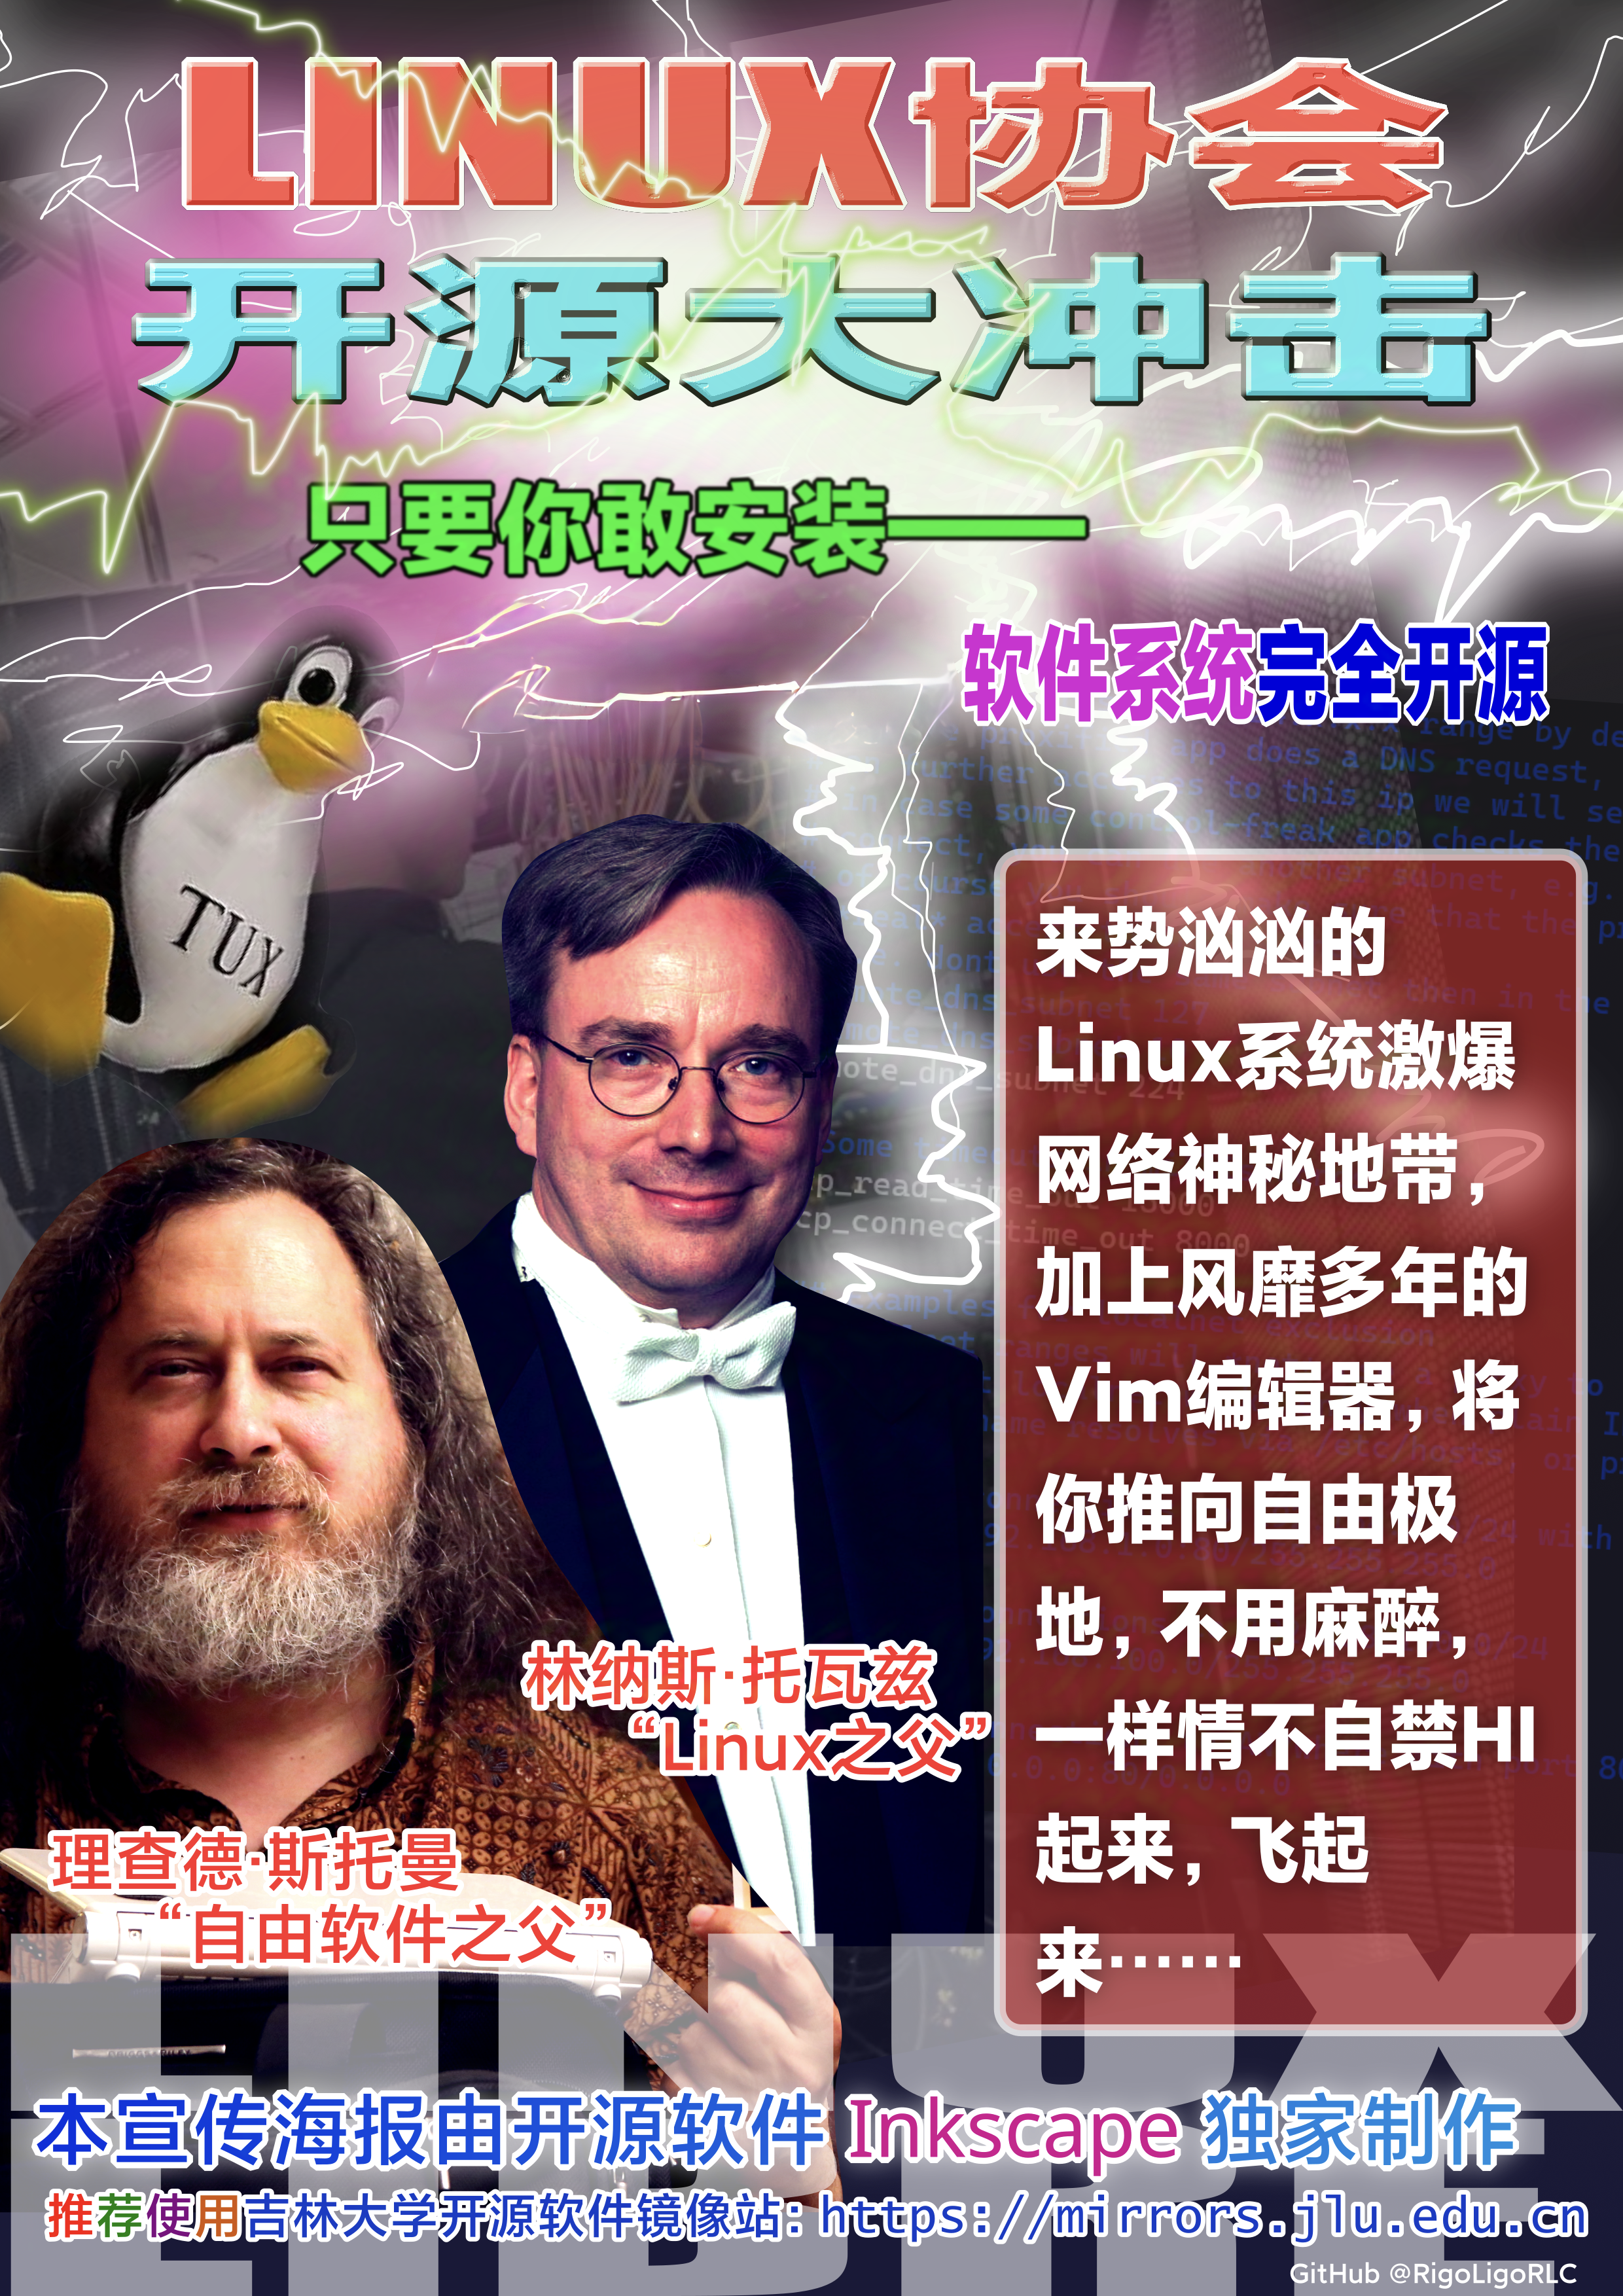
\includegraphics[width=\textwidth]{pic/!.png}
    \end{figure}
\end{column}
\end{columns}
\end{frame}

\begin{frame}{吉林大学开源镜像站}
    \begin{figure}[c]
        \centering
        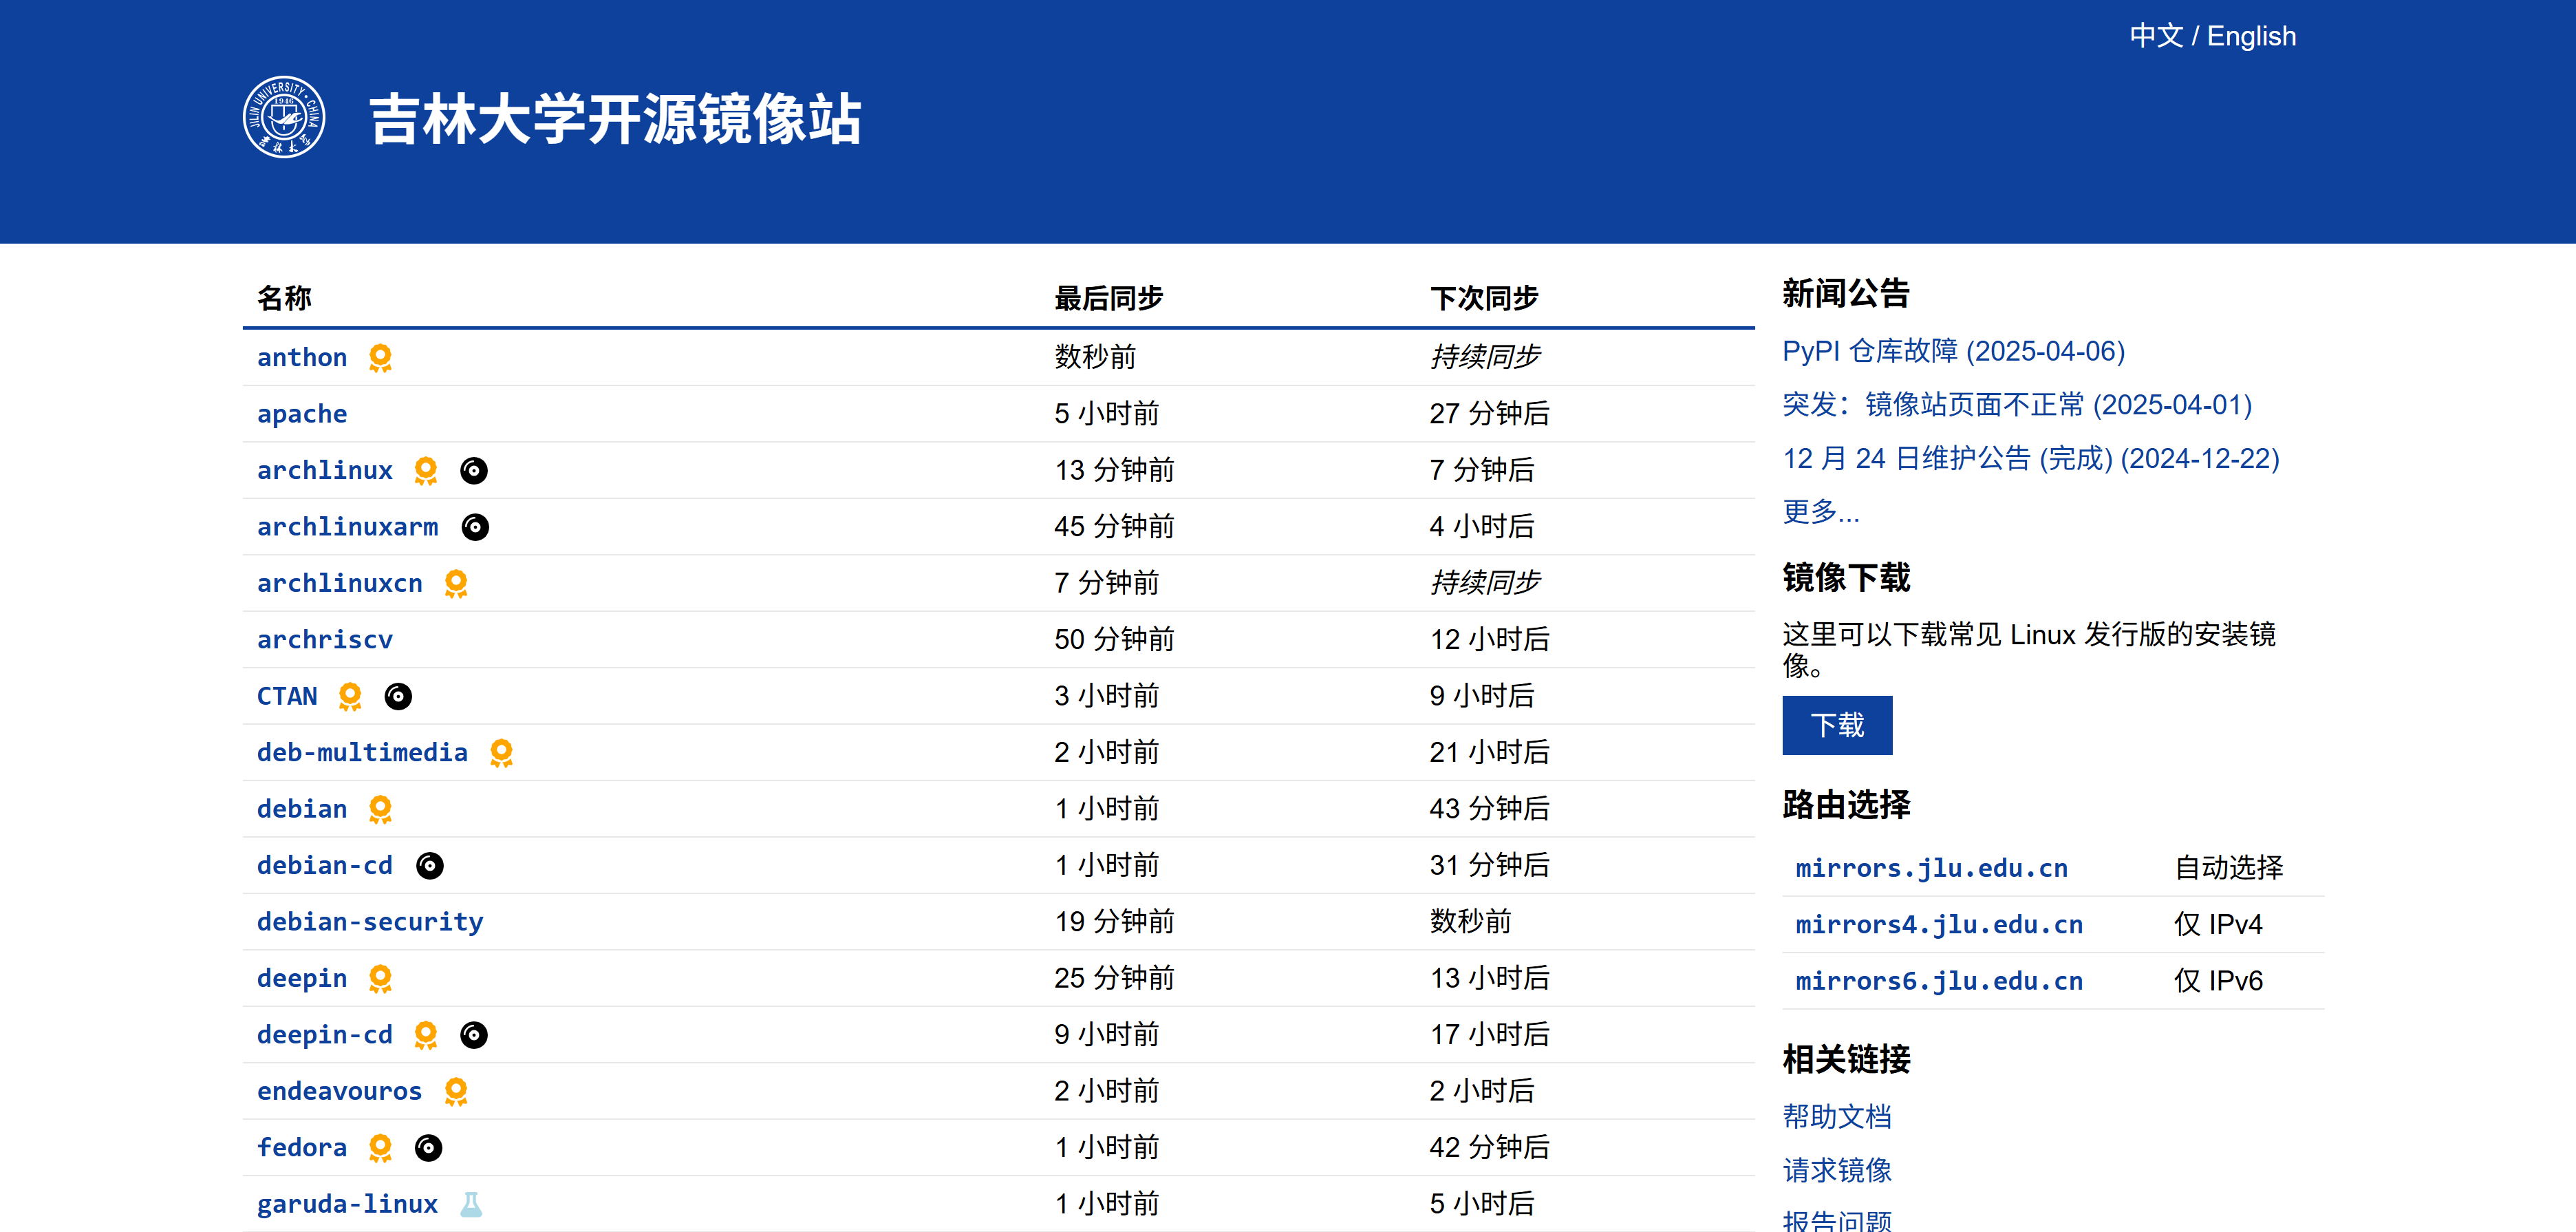
\includegraphics[width=\textwidth]{pic/mirrors.png}
        \caption{https://mirrors.jlu.edu.cn/}
    \end{figure}
\end{frame}

\section{常见发行版介绍}

\begin{frame}{Debian}
\begin{columns}
\begin{column}{0.7\textwidth}
    \begin{itemize}
        \item 1993 年 9 月，Debian GNU/Linux 0.01 问世.
        \item 最早期发行版之一，拥有大量的软件包资源.
        \item 坚持自由精神，基本不含有非自由成分.
        \item 稳定性优秀.
    \end{itemize}
\end{column}
\begin{column}{0.2\textwidth}
    \begin{figure}[c]
        \centering
        
\includegraphics[width=\textwidth]{pic/debian.png}
    \end{figure}
\end{column}
\end{columns}
\end{frame}

\begin{frame}{Ubuntu}
\begin{columns}
\begin{column}{0.8\textwidth}
    \begin{itemize}
        \item Debian 衍生版.
        \item 最早期发行版之一，拥有大量的软件包资源.
        \item 新手友好, 有较大的用户社区(帮你踩坑).
        \item 主要针对桌面应用环境适用.
    \end{itemize}
\end{column}
\begin{column}{0.2\textwidth}
    \begin{figure}[c]
        \centering
        
\includegraphics[width=1.2\textwidth]{pic/ubuntu.png}
    \end{figure}
\end{column}
\end{columns}
\end{frame}

\begin{frame}{\textbf{R}ed \textbf{H}at (\textbf{E}nterprise) \textbf{L}inux}
\begin{columns}
\begin{column}{0.8\textwidth}
    \begin{itemize}
        \item 由 Red Hat 公司发行的经典发行版.
        \item 社区版本: 1994 - 2003, R.I.P.
        \item 企业版本: 2002.03 - 至今
        \item 稳定性优秀的企业版 Linux. (前提是掏钱订阅支持服务.)
        \item 更新策略较为保守，可以使用 EPEL 补充新软件包.
    \end{itemize}
\end{column}
\begin{column}{0.2\textwidth}
    \begin{figure}[c]
        \centering
        
\includegraphics[width=1.2\textwidth]{pic/rh.png}
    \end{figure}
\end{column}
\end{columns}
\end{frame}

\begin{frame}{Fedora}
\begin{columns}
\begin{column}{0.8\textwidth}
    \begin{itemize}
        \item 由社群接管的 RHL 后继版本, 红帽资助.
        \item 更新策略较为激进，新特性较多，社区较活跃.
        \item 进入 RHEL 的新特性会先在 Fedora 中测试.
        \item Linus 本人钦定的发行版.
    \end{itemize}
\end{column}
\begin{column}{0.2\textwidth}
    \begin{figure}[c]
        \centering
        
\includegraphics[width=\textwidth]{pic/fedora.png}
    \end{figure}
\end{column}
\end{columns}
\end{frame}

\begin{frame}{\textbf{C}ommunity \textbf{Ent}erprise \textbf{OS}}
\begin{columns}
\begin{column}{0.8\textwidth}
    \begin{itemize}
        \item RHEL 源码重新编译 + 替换商标 = CentOS.
        \item 2020 年底，项目性质改变，下游变开发分支.
        \item Linus 本人钦定的发行版.
        \item 已经进入历史的垃圾堆.
    \end{itemize}
    \begin{figure}[c]
        \centering
        
\includegraphics[width=.8\textwidth]{pic/issue.png}
    \end{figure}
\end{column}
\begin{column}{0.2\textwidth}
    \begin{figure}[c]
        \centering
        
\includegraphics[width=1.2\textwidth]{pic/centos.png}
    \end{figure}
\end{column}
\end{columns}
\end{frame}

\begin{frame}{Rocky Linux}
\begin{columns}
\begin{column}{0.8\textwidth}
    \begin{itemize}
        \item 由 CentOS 创始人分裂出来, 坚持 CentOS 原本的目标, 由社群支持.
        \item 与 RHEL 保持 Bug 级兼容.
        \item 目前 CentOS EOL 后最流行的替代方案.
    \end{itemize}
\end{column}
\begin{column}{0.2\textwidth}
    \begin{figure}[c]
        \centering
        
\includegraphics[width=1.2\textwidth]{pic/rocky.png}
    \end{figure}
\end{column}
\end{columns}
\end{frame}

\begin{frame}{Arch Linux}
\begin{columns}
\begin{column}{0.7\textwidth}
    \begin{itemize}
        \item 始于 2002 年.
        \item 社区驱动, 独立开发, 滚动更新.
        \item Arch 哲学: 简洁, 现代, 实用, 人本, 万能.
        \item user-centric v.s. user-friendly.
        \item 安装后只含最小系统，其他一切自己装.
        \item 豪华文档: ArchWiki.
    \end{itemize}
\end{column}
\begin{column}{0.3\textwidth}
    \begin{figure}[c]
        \centering
        
\includegraphics[width=1.2\textwidth]{pic/arch.png}
    \end{figure}
\end{column}
\end{columns}
\end{frame}

\begin{frame}{Manjaro}
\begin{columns}
\begin{column}{0.8\textwidth}
    \begin{itemize}
        \item 始于 2011 年的 Arch 衍生版.
        \item 旨在解决 Arch 过于用户不友好的问题, 默认提供图形化界面, 安装向导, 显卡驱动.
        \item 适合想了解 Arch 生态的新手使用.
    \end{itemize}
\end{column}
\begin{column}{0.2\textwidth}
    \begin{figure}[c]
        \centering
        
\includegraphics[width=1.2\textwidth]{pic/manjaro.png}
    \end{figure}
\end{column}
\end{columns}
\end{frame}

\begin{frame}{NixOS}
\begin{columns}
\begin{column}{0.7\textwidth}
    \begin{itemize}
        \item 始于 2003 年.
        \item 独树一帜的包管理方式: Nix.
        \item 声明式, 函数式, 可复现的操作系统?
        \item 软件包最丰富的发行版(之一).
        \item 非 FHS 发行版?
        \item 文档缺失? Flakes or not?
    \end{itemize}
\end{column}
\begin{column}{0.3\textwidth}
    \begin{figure}[c]
        \centering
        
\includegraphics[width=1.2\textwidth]{pic/nixos.png}
    \end{figure}
\end{column}
\end{columns}
\end{frame}

\begin{frame}{AOSC OS}
\begin{columns}
\begin{column}{0.7\textwidth}
    \begin{itemize}
        \item 中文社区独立构建和维护的操作系统.
        \item 简化精制, 非必要不拆分软件包.
        \item 对开源, 闭源, Wine 软件一视同仁.
        \item 部署快捷, 开箱即用, 但建议有基础.
        \item 支持 LoongArch (龙架构), x86-64, AArch64 等架构.
    \end{itemize}
\end{column}
\begin{column}{0.3\textwidth}
    \begin{figure}[c]
        \centering
        
\includegraphics[width=1.2\textwidth]{pic/aosc.png}
    \end{figure}
\end{column}
\end{columns}
\end{frame}

\begin{frame}{特定用途的发行版}
\begin{columns}
\begin{column}{0.6\textwidth}
    \begin{itemize}
        \item Kali Linux, BlackArch Linux: 用于渗透测试和数字鉴识.
        \item SteamOS: 用于 Steam Deck.
        \item Android: 用于智能手机.
        \item OpenWRT: 用于路由器等网络设备.
    \end{itemize}
\end{column}
\begin{column}{0.2\textwidth}
    \begin{figure}[c]
        \centering
        
\includegraphics[width=1.2\textwidth]{pic/kali.png}
    \end{figure}
    \begin{figure}[c]
        \centering
        
\includegraphics[width=.8\textwidth]{pic/android.png}
    \end{figure}
\end{column}
\begin{column}{0.2\textwidth}
    \begin{figure}[c]
        \centering
        
\includegraphics[width=.8\textwidth]{pic/blackarch.png}
    \end{figure}
    \begin{figure}[c]
        \centering
        
\includegraphics[width=1.2\textwidth]{pic/openwrt.png}
    \end{figure}
\end{column}
\end{columns}
\end{frame}

\section{现场安装 Linux 发行版}

\begin{frame}{GNU/Linux 常见桌面环境介绍}
    \begin{itemize}
        \item 桌面环境向用户提供一系列显示基础设施和实用程序.
        \item GNOME: 基于 GTK4 框架开发, 圆角较大, 触摸/手势交互体验较好.
        \item KDE Plasma: 基于 Qt 框架开发, 圆角比较少.
        \item Xfce: 基于 GTK3 框架开发, 轻量级，占用资源极少.
        \item LXDE: 轻量级桌面环境, 为低性能设备定制.
    \end{itemize}
\end{frame}

\begin{frame}{Linux 的安装方式}
    \begin{itemize}
        \item 从云服务商租用一台云服务器.
        \item 使用虚拟机安装.
        \begin{itemize}
            \item 使用一般虚拟机软件安装.
            \item 使用 WSL (Windows Subsystem for Linux).
        \end{itemize}
        \item 直接物理机安装.
        \begin{itemize}
            \item 双系统.
            \item 单系统.
        \end{itemize}
    \end{itemize}
\end{frame}

\begin{frame}
    \begin{center}
        {\Huge\calligra Talk is Cheap,}
    \end{center}
    \begin{center}
        {\Huge\calligra Let’s Install Linux!}
    \end{center}
\end{frame}

\end{document}
